\title{\bf Lecture 9 - Dao\\}
\author{\bf Rylan Schaeffer and Vincent Yang\\}
\date{\bf \today \\}

\documentclass{article}
\renewcommand{\thesubsection}{\thesection.\alph{subsection}}
\usepackage{enumerate}
\usepackage{listings}
\usepackage{amsmath}
\usepackage{graphicx}
\setlength{\oddsidemargin}{0in}
\setlength{\evensidemargin}{0in}
\setlength{\textheight}{9in}
\setlength{\textwidth}{6.5in}
\setlength{\topmargin}{-0.5in}

\begin{document}
\maketitle

Note: This lecture is based on Princeton University's BTC-Tech: Bitcoin and Cryptocurrency Technologies Spring 2015 course.

\section*{ZKP Continued}
\begin{itemize}
  \item Billard Balls: Alice is blind and has two billard balls. Bob claims that these two billard balls are of different color, but Alice doesn't believe him.
    What is a ZKP that Alice can use in order to distinguish if the two billard balls are really of different color?
  \item Other:
    \subitem Bridge 1, 2, 5, 10, 17
    \subitem 1000 wine
    \subitem Light switches
\end{itemize}

\section*{DAO}
\begin{itemize}
  \item People crowdfunded \$150 million into the DAO, also called the Decentralized Autonomous Organization
    \subitem This can be compared to the Pebble Watch, which had \$20 million raised
    \subitem \$30 million in the first 10 days
  \item In a normal company, any decision is made by whoever has the authority - CEO, Board of Directors, etc.
    \subitem Instead, the DAO functions similarly to shareholder rights in a company. Through DAO tokens, you can 
    \begin{enumerate}
      \item Submit proposals for funding
      \item Vote on which proposals are funded
      \item Receive profits from funded projects
    \end{enumerate}
  \item Big promise: new way to manage and allocate capital
    \subitem Capital Allocation without a fund manager
  \item Backed up by 11,000 anonymous stakeholders who can vote on any major decision to spend funds
  \item Any company or individual who would like to use funds have to submit a proposal, which is then published online
  \item After these are published online, stakeholders vote on adoption - aka whether or not to allocate some of the \$150 million
    or not
  \item Contractors submit Proposals for the development of products or services - these are written in English, then code
    \subitem DAO Token Holders can pull the plug on funding anytime, subject to the Proposal
  \item 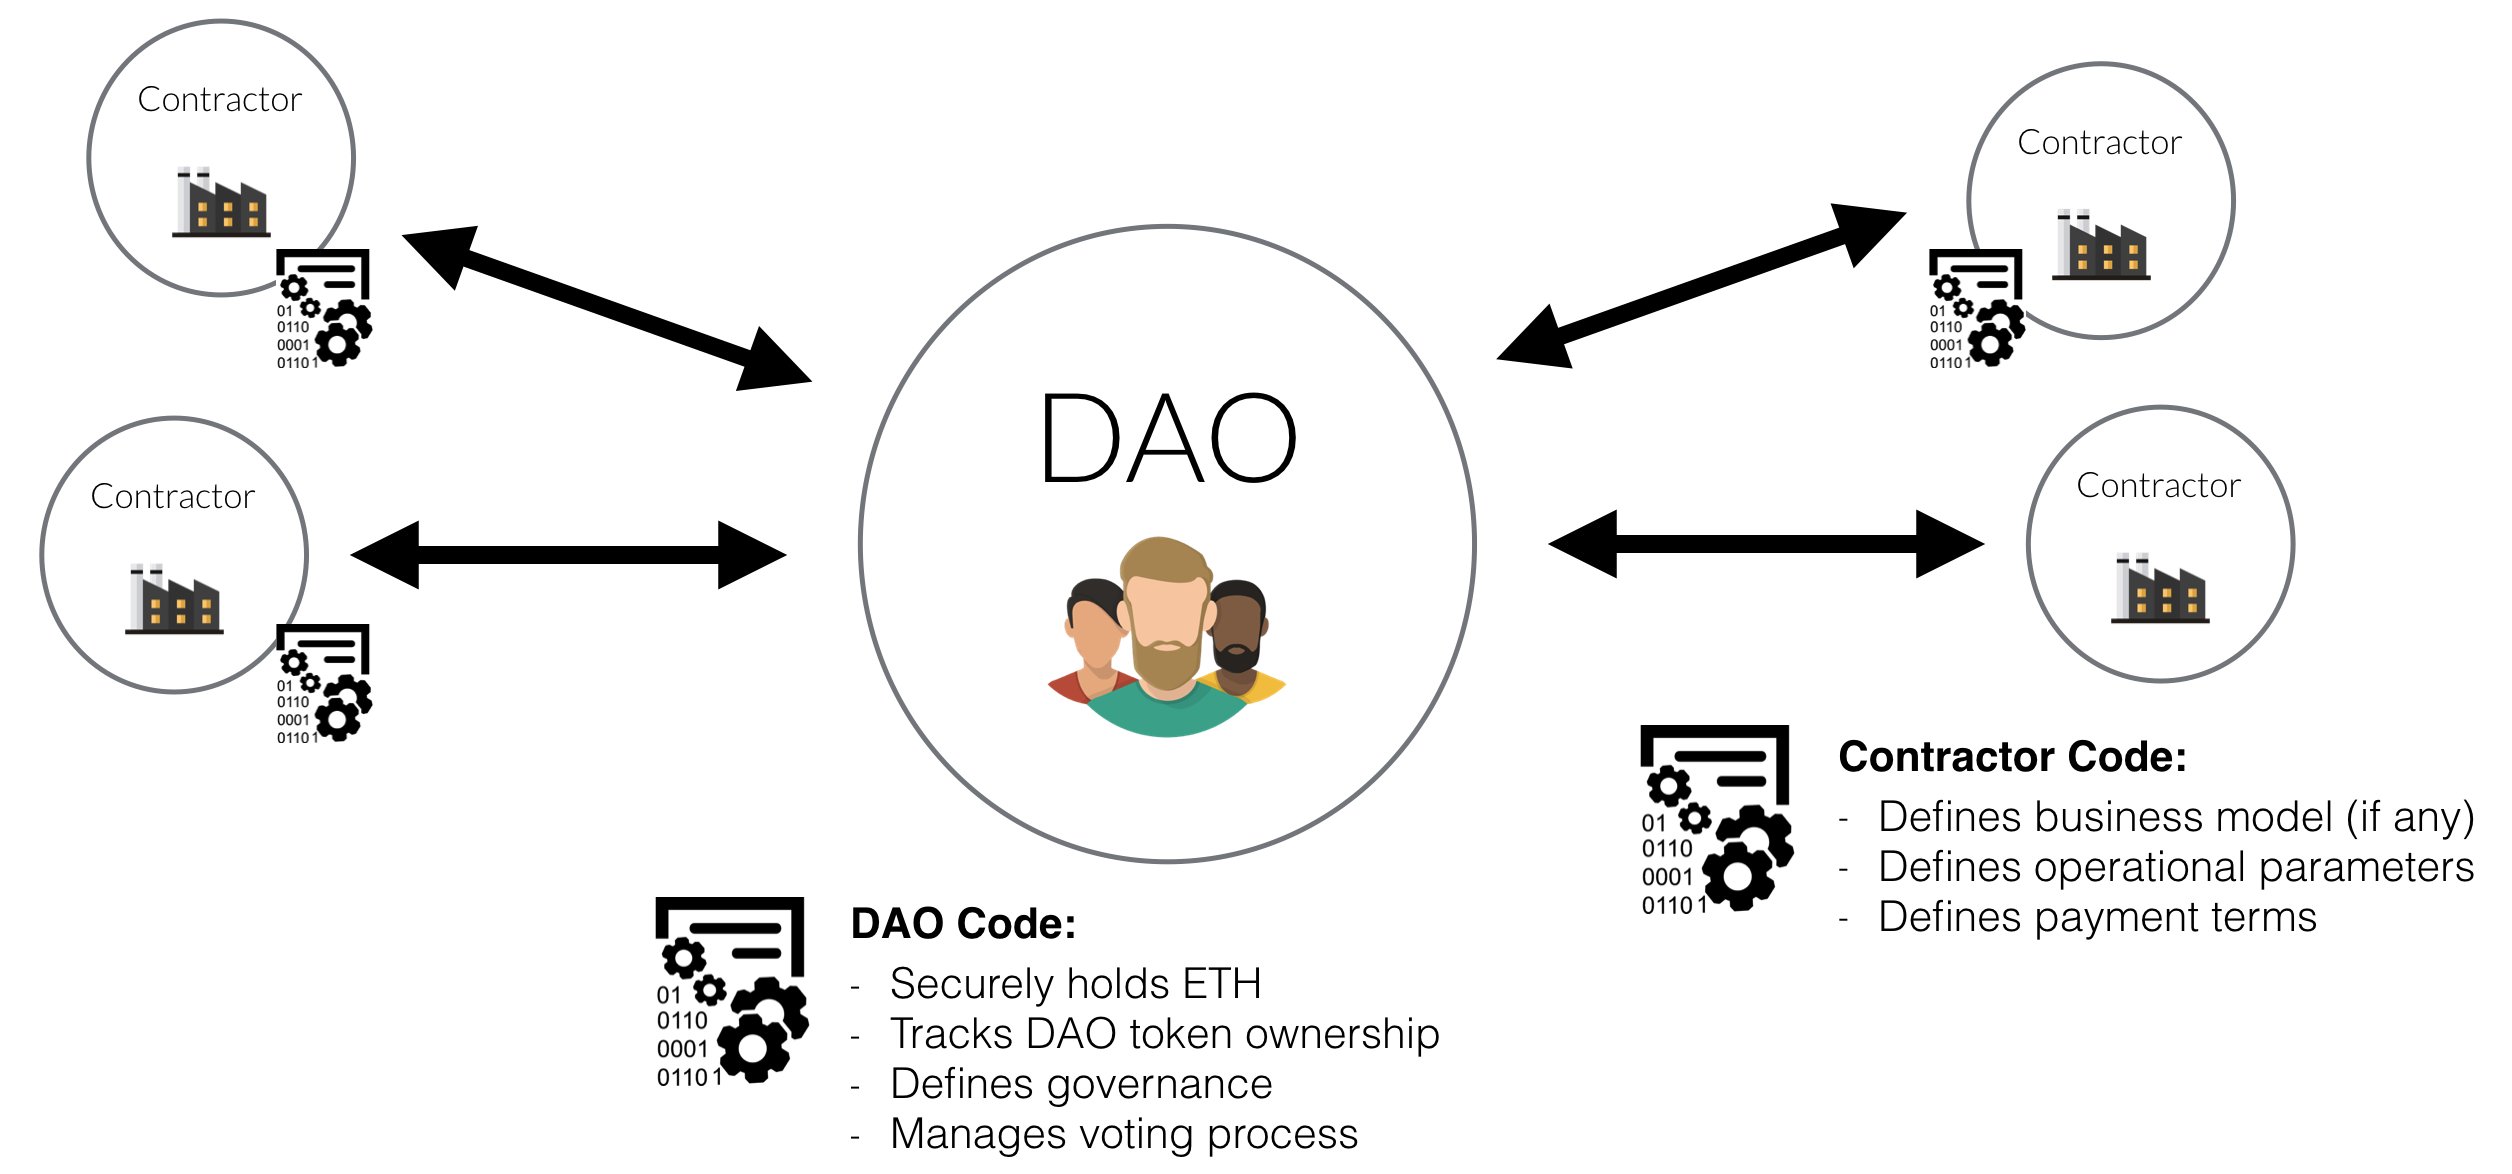
\includegraphics[width=4in]{independence.png}\\
  \item 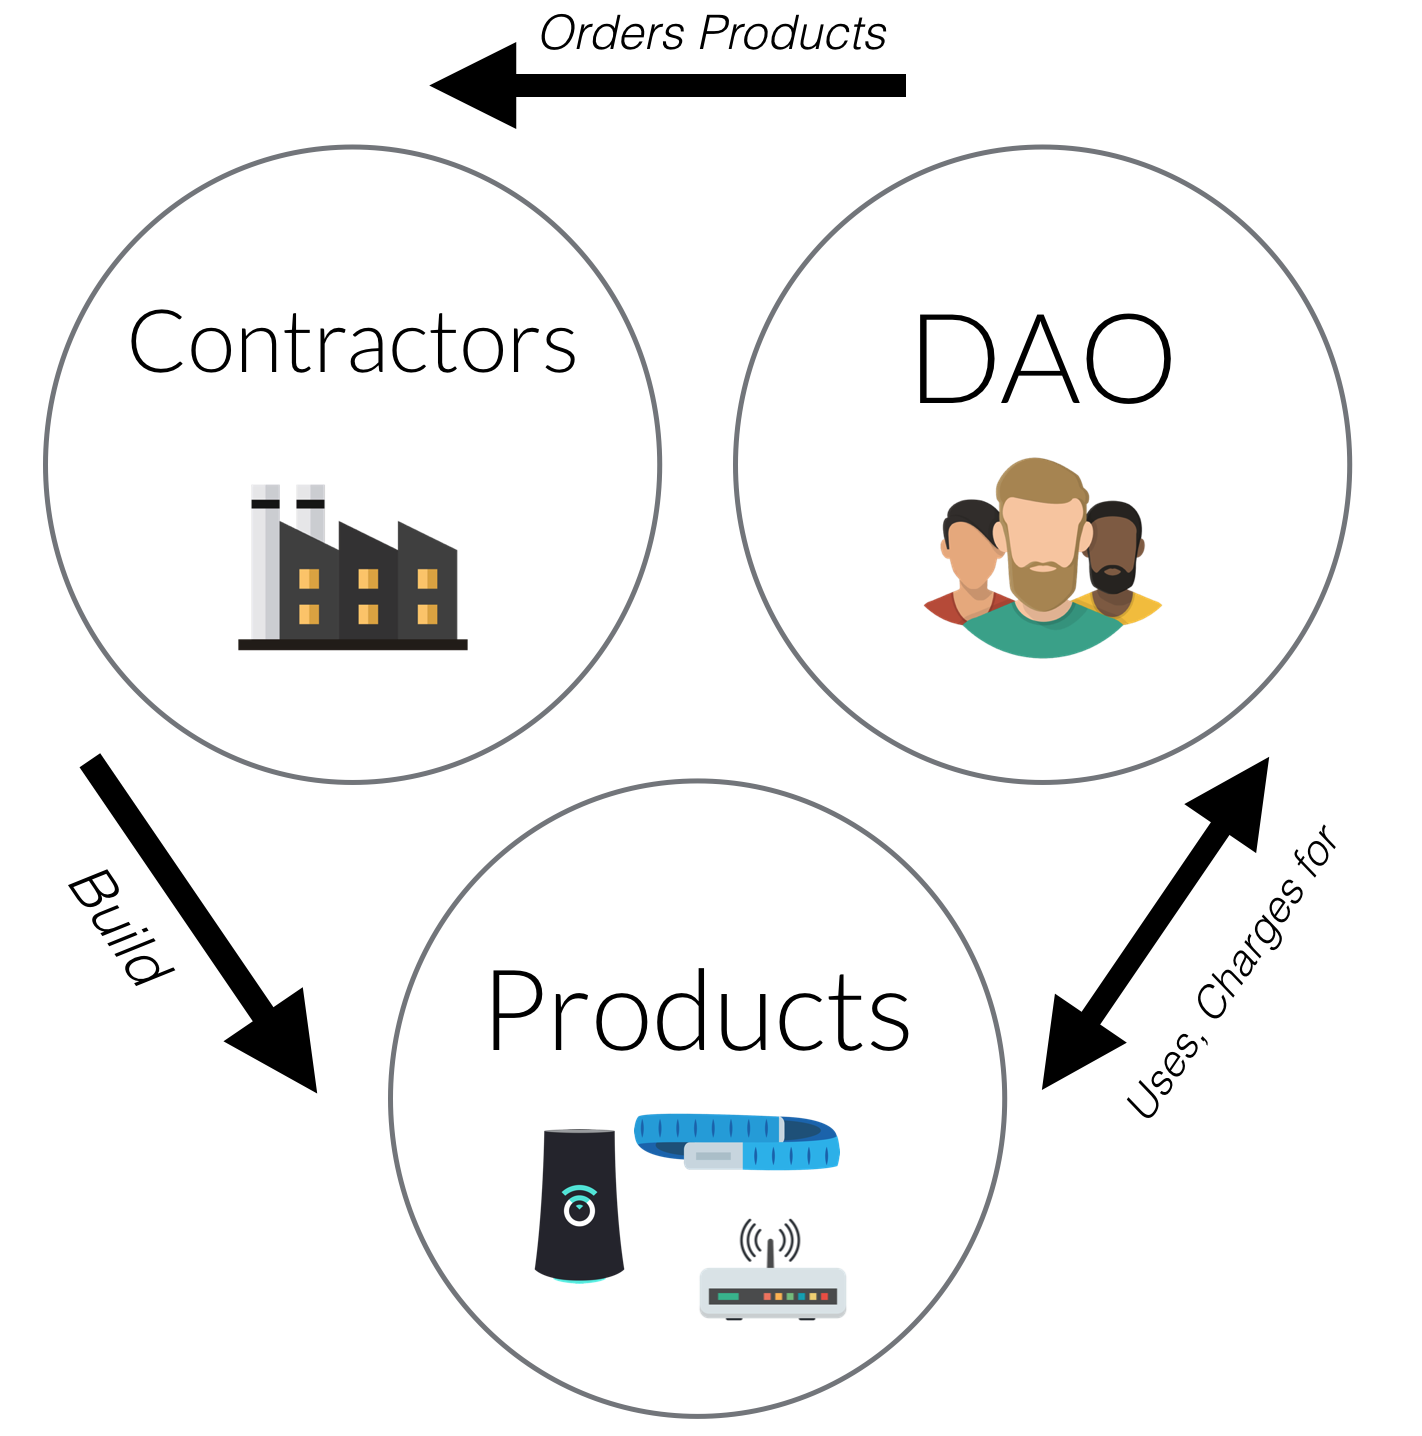
\includegraphics[width=4in]{synergistic.png}\\
  \item The only centralized aspect is the Curators who play an escrow role
    \subitem Escrow: financial aspect held by 3rd party on behalf of the other 2 for a transaction
    \begin{itemize}
      \item This is a failsafe to prevent a 51\% attack. Rather than adding centralization to the DAO, they're nominated by token holders and can be
        fired any time for any reason. 
      \item Curators curate the whitelist, which is the list of Contractors authorized to receive ether from the DAO.
      \item Serve two functions:
        \begin{enumerate}
          \item When a DAO Token Holder submits a Proposal in the form of a smart contract, the Curator checks that the published contract on the Ethereum blockchain
            matches the source that the Contractor says they've deployed (compare bytecode)
          \item Second, a Curator confirms the origin of a Proposal, This is done by having the submitting entity send a signed transaction with a set of data known only to the
            Curator and the author of the proposal.
        \end{enumerate}
      \item Now, the following are functions of the DAO as a whole, not the Curator.
        \subitem Evaluate how good a Proposal is
        \subitem Audit smart contract code
        \subitem Provide legal advice
        \subitem Take responsibility for the proposal
      \item This is done by a multisig involving Vitalik Buterin (Inventor and Founder), Alex Van de Sande (Chief Designer), and other highly involved individuals
      \item Changing the Curator:
        \begin{itemize}
          \item Changing the Curator takes the form of a Proposal with a special flag
          \item Votes take place in two steps: First, a non binding vote on whether or not DAO Token Holders would like to switch Curators, then
            second, a confirmation vote to give a chance to DAO Token Holders a chance to confirm or deny the result of the first vote. If the minority chooses to split, 
            they may do so, similar to how a company might split in two
        \end{itemize}
      \item The huge advantage of having Curators is that even with a 51\% attack, someone can't make a proposal sending themself 100\% of the DAO's ETH.

    \end{itemize}
  \item This is so big such that it now accounts for 14\% of all Ether for Ethereum.
  \item Stakeholders are incentivized since they can potentially gain from their slice of the profits
  \item Proposals:
    \begin{itemize}
      \item Stephan Tual is the chief executive of Slockit, which is a company with a proposal for funding from DAO that's played a large role
        in getting DAO going
        \subitem Slockit's CTO wrote a good portion of the code for DAO. This combines IOT with Blockchain
        \subitem Basically if you can lock it, you can rent, sell, or share it. 
        \subitem IOT opening and closing locks based on smart contracts
        \subitem For instance, they could control access to cars, bikes, and storage units. 
        \subitem Cars could be parked in roads waiting for the customer, then opened with an app
    \end{itemize}
    \begin{itemize}
      \item Mobotiq
        \begin{itemize}
          \item Problem: Fossil fuel addiction is a large cause for pollution, global warming, geopolitical tensions, and terrorism
            \subitem Old product: polluted the Earth, inefficient, high cost per km, planned obsolescence
            \subitem Old organization: closed, innovation aversive
            \subitem Old manufacturing system: centralized mass production with high barriers to entry
            \subitem Old business model based on ownership
          \item Solution: Create a new supply and demand ecosystem
            \subitem New product: clean, efficient, affordable, designed to last, software intensive, modular, simple
            \subitem New organization: open, innovation friendly networked meritocracy
            \subitem New manufacturing system: distributed without barriers to entry
            \subitem New business model: demand centric, based on p2p rentership
          \item Modular parts for transportation that doesn't rely on gas
          \item DIY  mindset - people can assemble modular components with different configurations
          \item Current prototype: tested to be safer than a conventional car
          \item 1 m width, so it can lane split
          \item Designed to lean in curves
          \item Swap and carry battery with wall charger
          \item Connected with IOT - everything is monitored by sensors and cameras, so you can record and understand how each part works
            with every other part
          \item P2P Rental by design, so this is actually designed to be coupled with slock.it so you can rent it to others
          \item Designed to be driverless as well while being modular - it has parts for traction, steering, suspension, brakes, and tilting
        \end{itemize}
    \end{itemize}
  
\end{itemize}

\end{document}
